%!TEX root = ../Thesis.tex
\section{Beschreibung des Projektverlaufs}
\fancyhead[R]{Beschreibung des Projektverlaufs}
\label{instal}

\subsection{Tatsächliche Aufgabenverteilung im Team (Fabia Schmid)}
%%%%%%%%%%%
%Fabia
%%%%%%%%%%%

\begin{longtable}{|p{4cm}|p{10cm}|}
\hline
{\textbf{Name}} & {\textbf{Aufgaben}}  \\ \hline
Ruthild Gilles & Erstellung Service-Klassen,

Schreiben eines Protokolls,

Latex-Beauftragte,

Projekttagebuch führen, 

Dokumentation anfertigen \\ \hline 
Fabia Schmid  & Projektsteuerung und -planung, 

Erstellung der Layouts für die ActivityOverview,  

Erstellung der OnClickListener für die ActivityOverview,  

Projekttagebuch führen, 

Dokumentation anfertigen \\ \hline

Jan Beilfuß & Datenbankzugriffe, 

Start-Up-Lade-Routine von Note, 

Bilderhandling in Note und generell, 

Note-Applicationlogicstrukturierung, 

Unterstützung im Umgang mit Git, 

Mockdatenerstellung,

Projekttagebuch führen, 

Dokumentation anfertigen \\ \hline
Yannick Rüttgers & Erstellung ActivityOverview,  

Planung der Navigation zwischen Klassen, 

Erster Latexentwurfprojekttagebuch, 

Latex-Beauftragter, 

Projekttagebuch führen, 

Dokumentation anfertigen \\ \hline
Robin Menzel & Zusammenführung des Quellcodes, 

Administration der Versionsverwaltung,

Planung der Layouts,

Hilfe bei der Aufteilung von den Activities,

Erstellung des Mockups, 

Erstellung der Event Activity, 

Projekttagebuch führen, 

Dokumentation anfertigen \\ \hline
Florian Rath  & Aufteilung der Activities, 

Erstellung Activity ToDo, 

Projekttagebuch führen, 

Dokumentation anfertigen \\ \hline
Joscha Nassenstein & Erstellung von Note, 

Erstellung der TEN-Klassen,  

Erstellung Datendiagramm, 

Projekttagebuch führen, 

Dokumentation anfertigen \\ \hline
Sertan Cetin &  Aufteilung der Activities, 

Erstellung Activity ToDo, 

Projekttagebuch führen, 

Dokumentation anfertigen \\ \hline
\end{longtable}

\newpage
\subsection{Teammeetingprotokolle}
%%%%%%%%%%%
%Ruthild
%%%%%%%%%%%

\begin{figure}[H]
\centering
\begin{minipage}[t]{1\textwidth} % Breite, z.B. 1\textwidth		
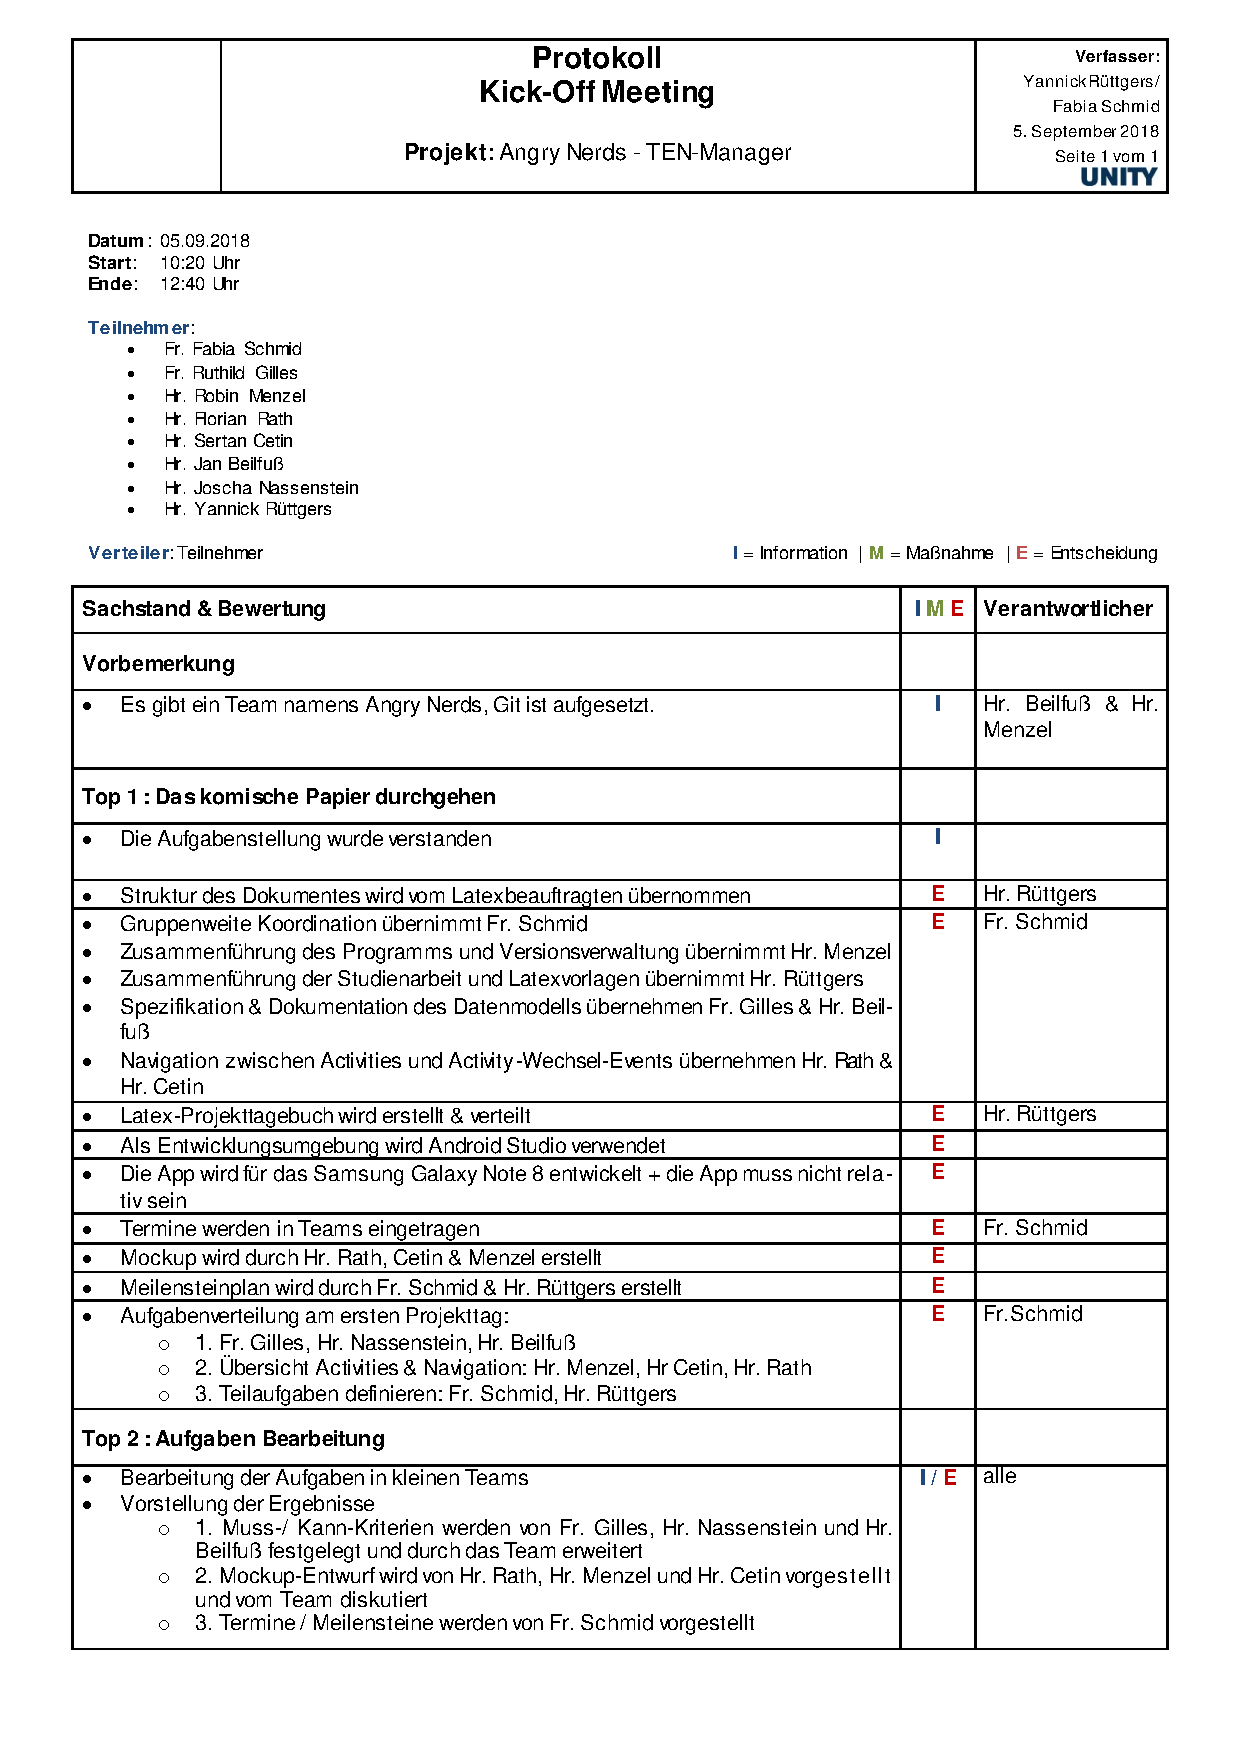
\includegraphics[height=20.5cm]{img/Protokoll2018-09-05.pdf}\\ % Pfad
\end{minipage}
\end{figure}

\begin{figure}[H]
\centering
\begin{minipage}[t]{1\textwidth} % Breite, z.B. 1\textwidth		
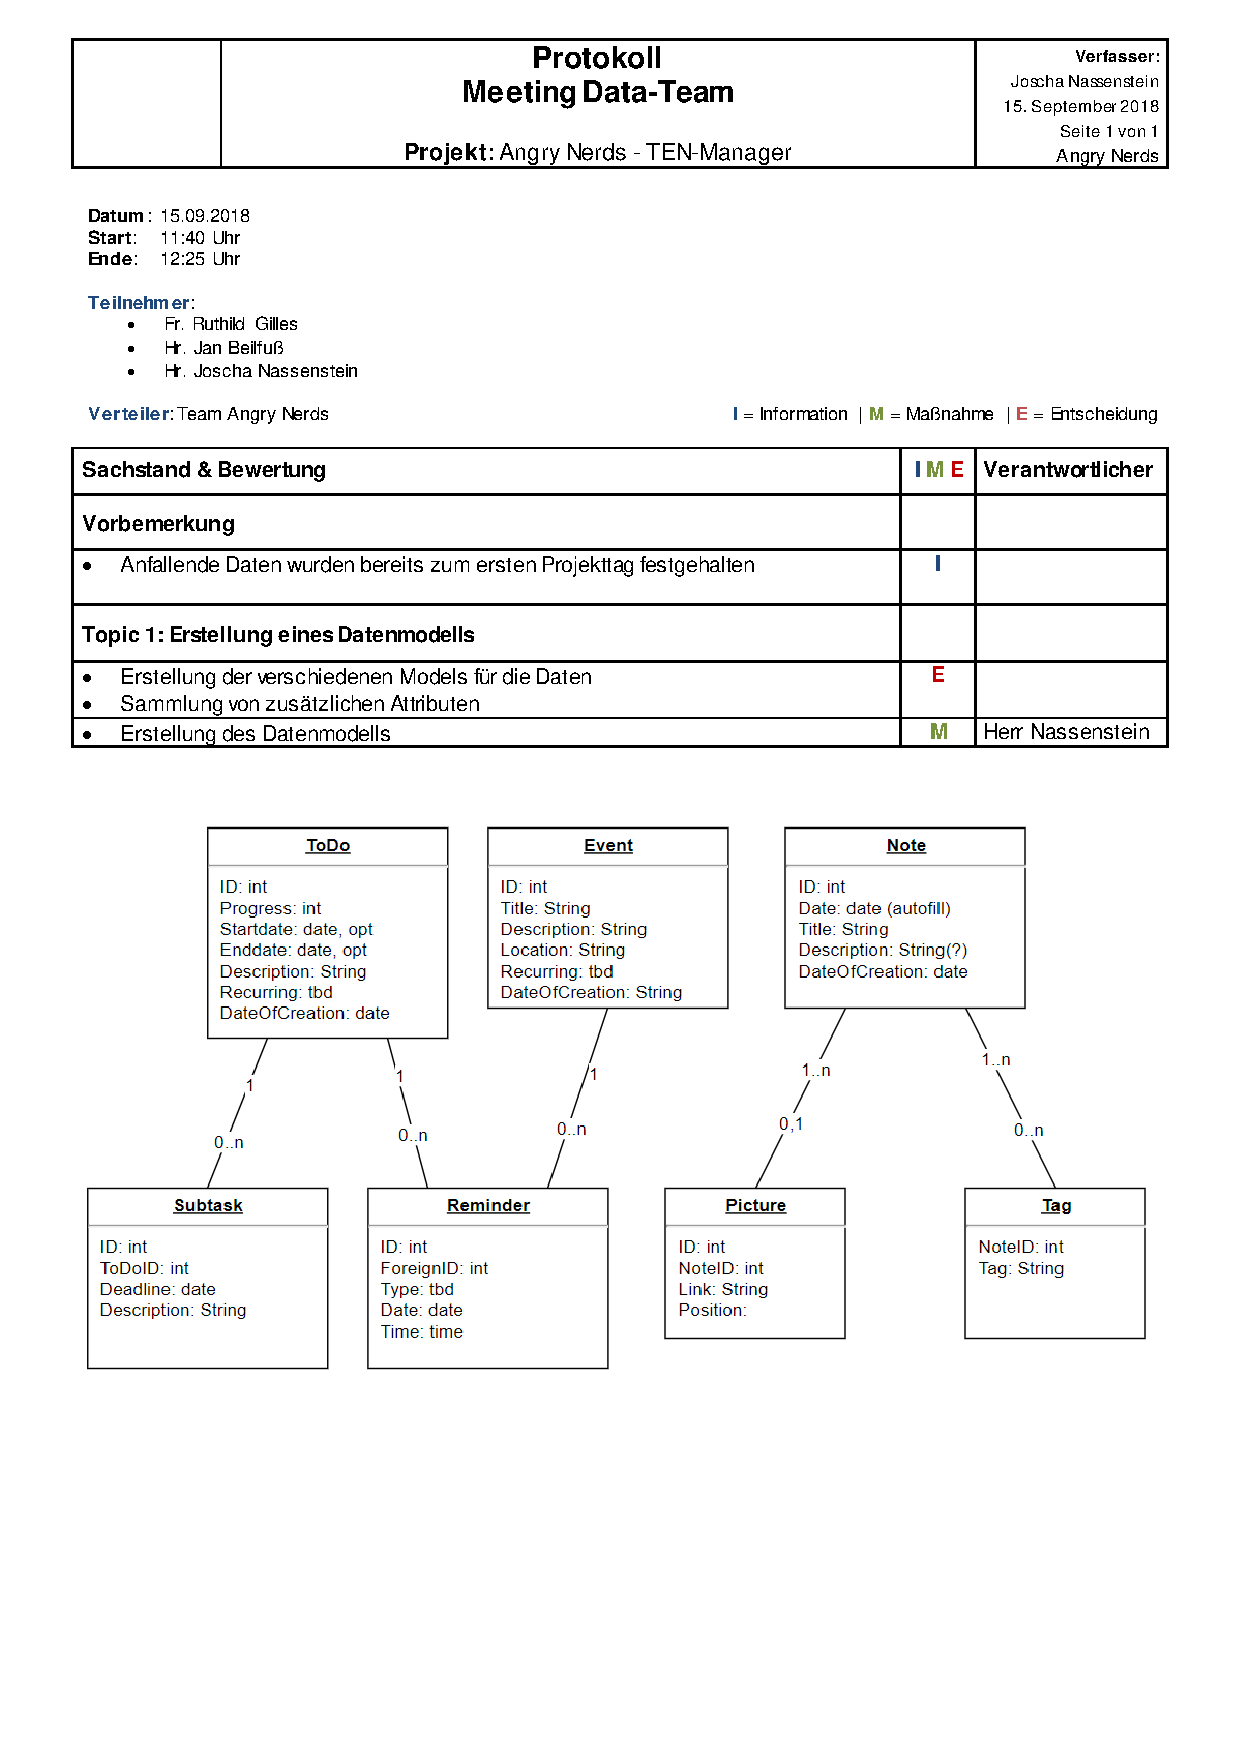
\includegraphics[width=1\textwidth]{img/Protokoll-DataTeam2018-09-15.pdf}\\ % Pfad
\end{minipage}
\end{figure}

\begin{figure}[H]
\centering
\begin{minipage}[t]{1\textwidth} % Breite, z.B. 1\textwidth		
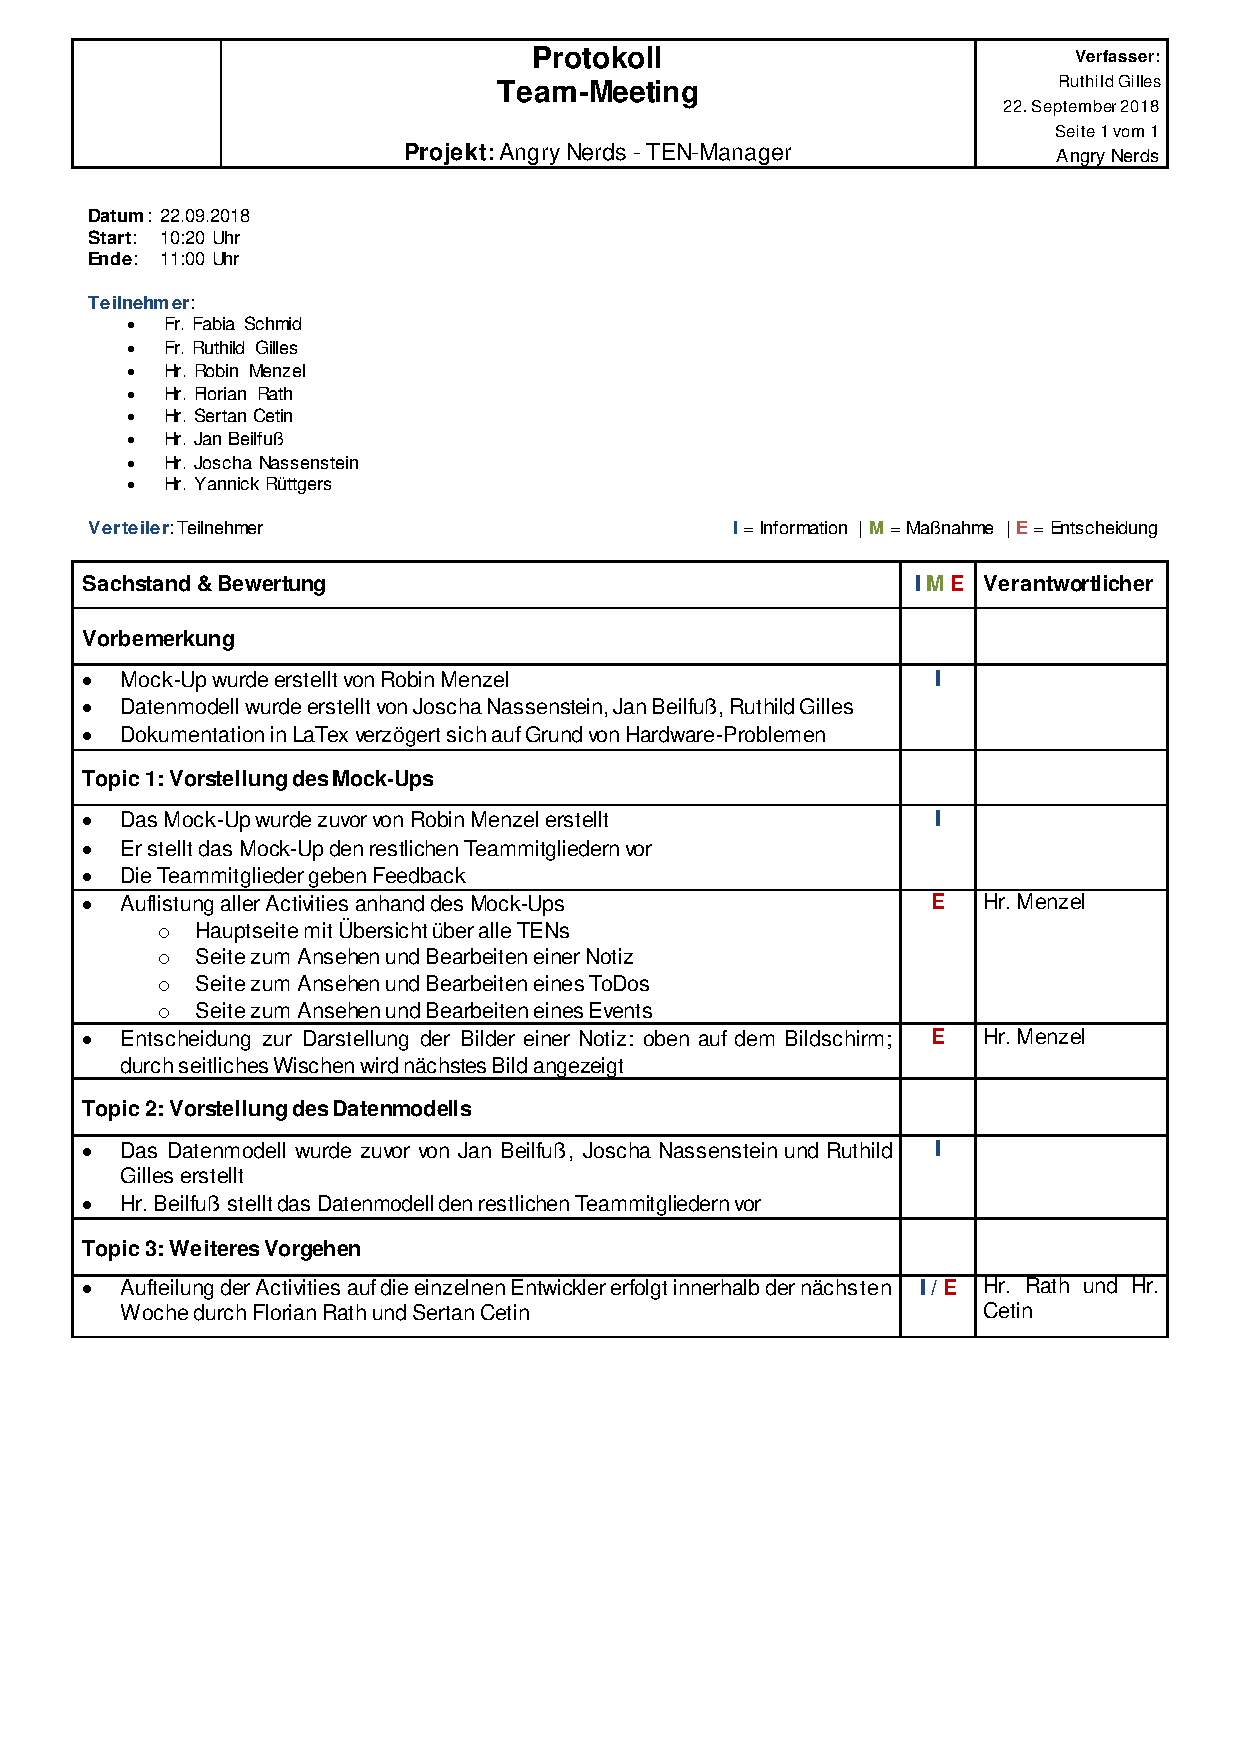
\includegraphics[width=1\textwidth]{img/Protokoll2018-09-22.pdf}\\ % Pfad
\end{minipage}
\end{figure}

\begin{figure}[H]
\centering
\begin{minipage}[t]{1\textwidth} % Breite, z.B. 1\textwidth		
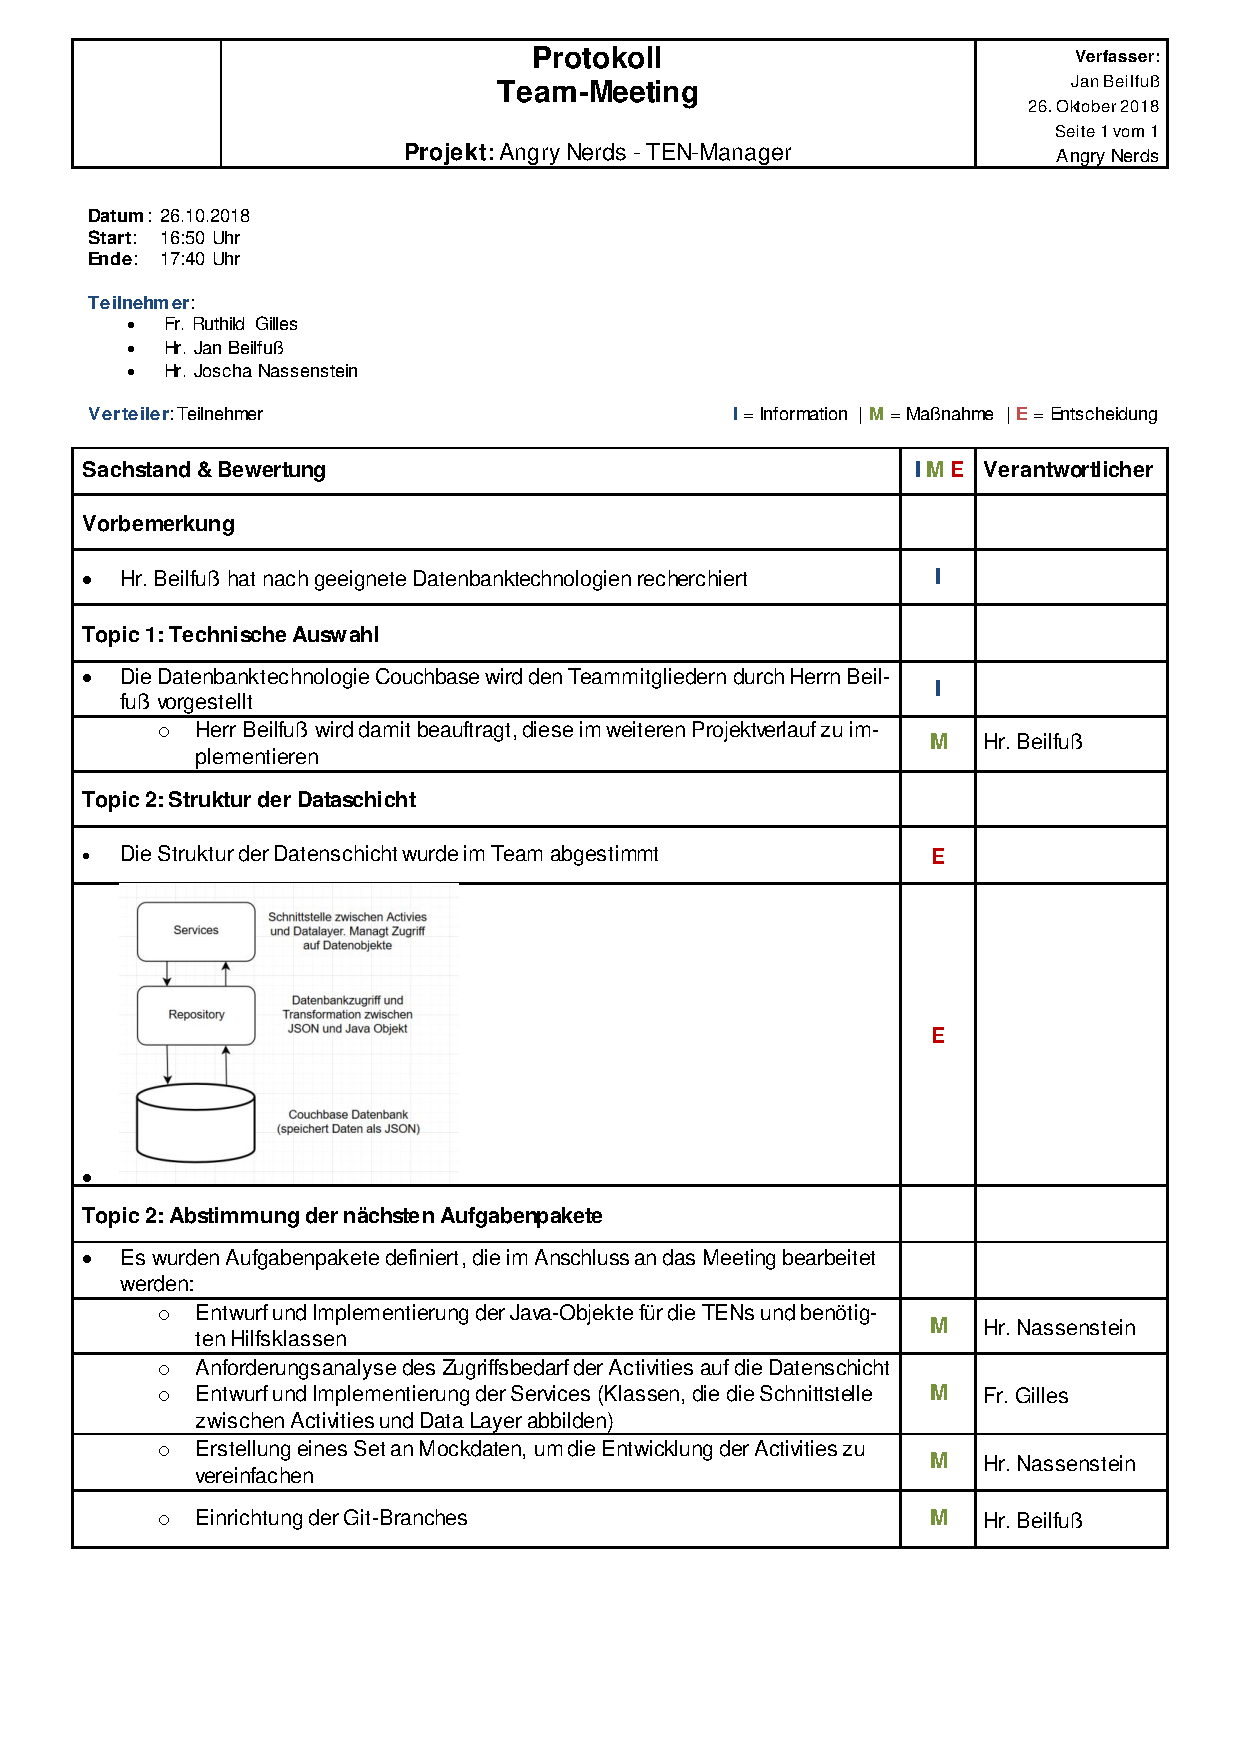
\includegraphics[width=1\textwidth]{img/Protokoll-DataTeam2018-10-26.pdf}\\ % Pfad
\end{minipage}
\end{figure}

\begin{figure}[H]
\centering
\begin{minipage}[t]{1\textwidth} % Breite, z.B. 1\textwidth		
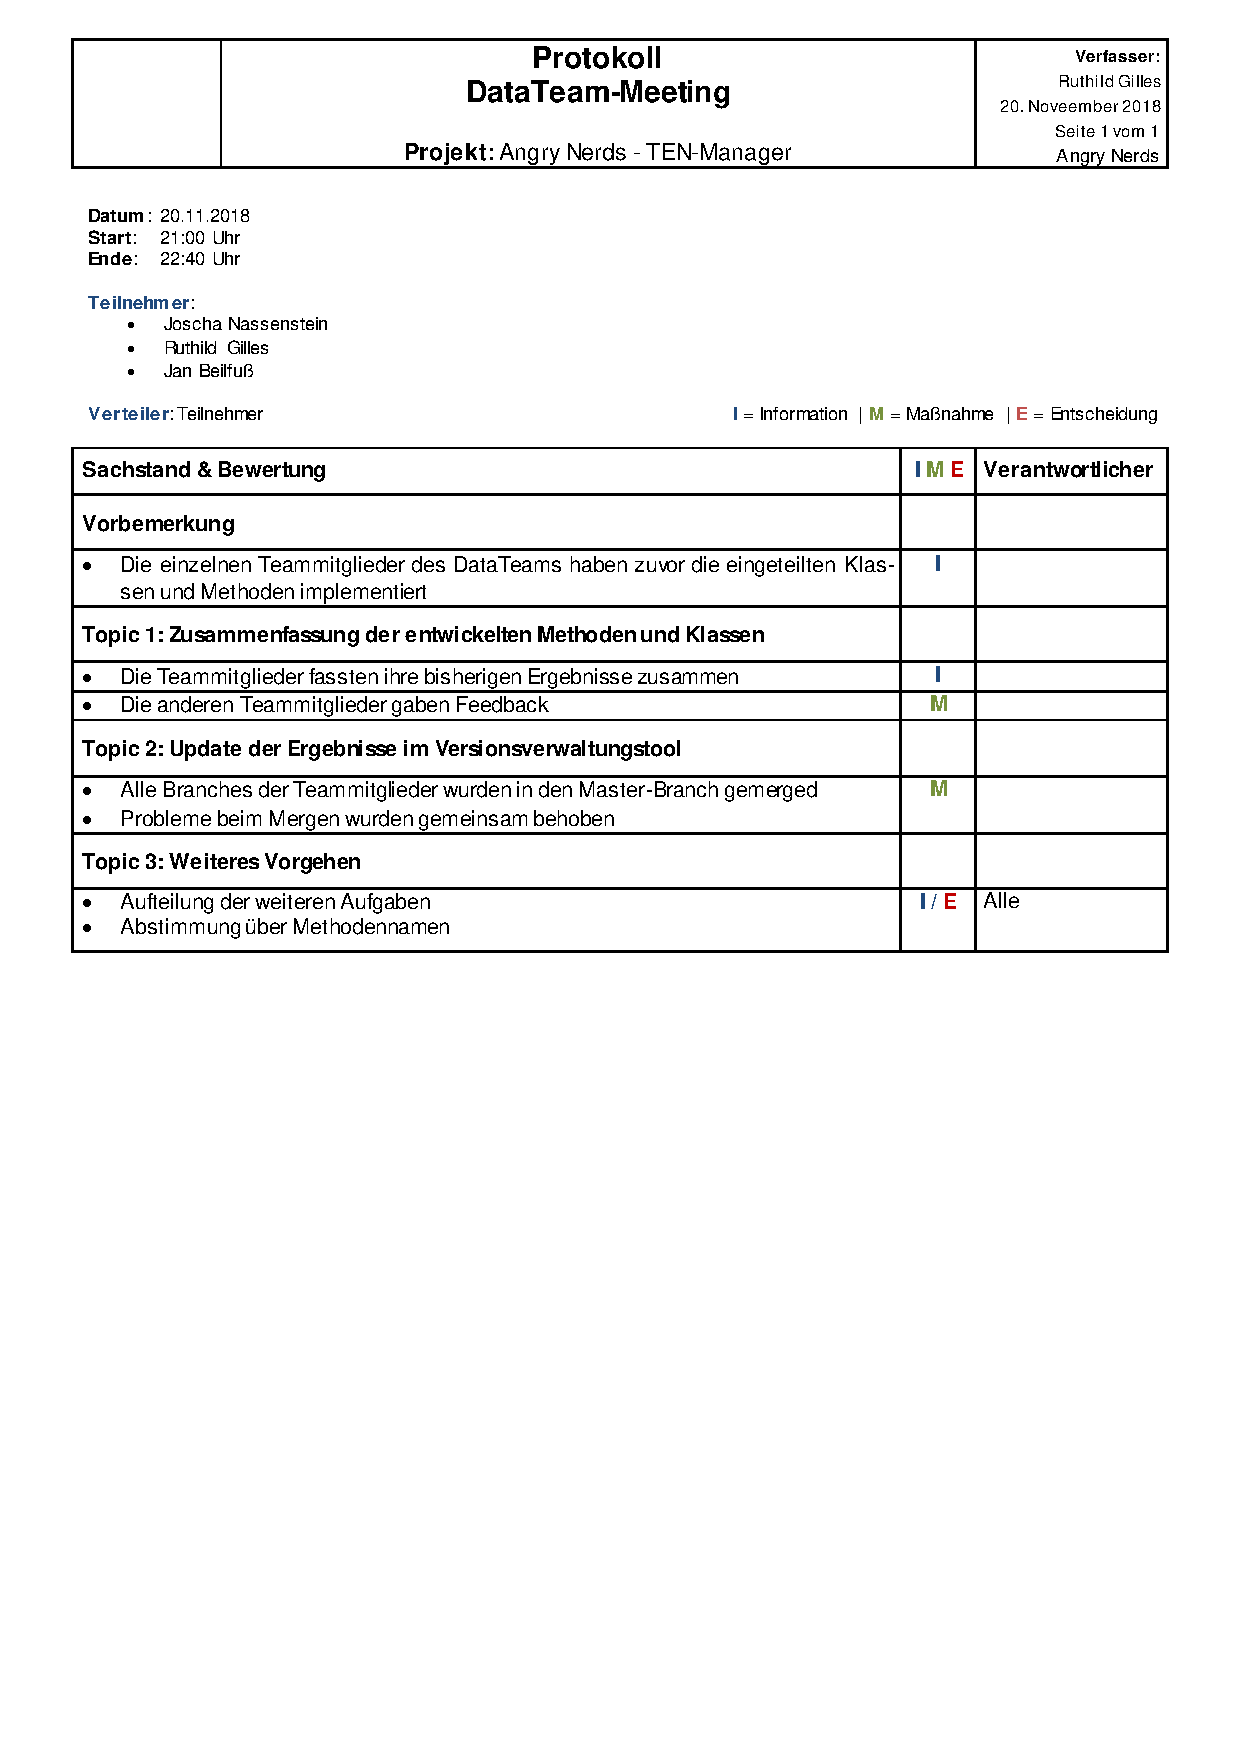
\includegraphics[width=1\textwidth]{img/Protokoll-DataTeam2018-11-20.pdf}\\ % Pfad
\end{minipage}
\end{figure}

\begin{figure}[H]
\centering
\begin{minipage}[t]{1\textwidth} % Breite, z.B. 1\textwidth		
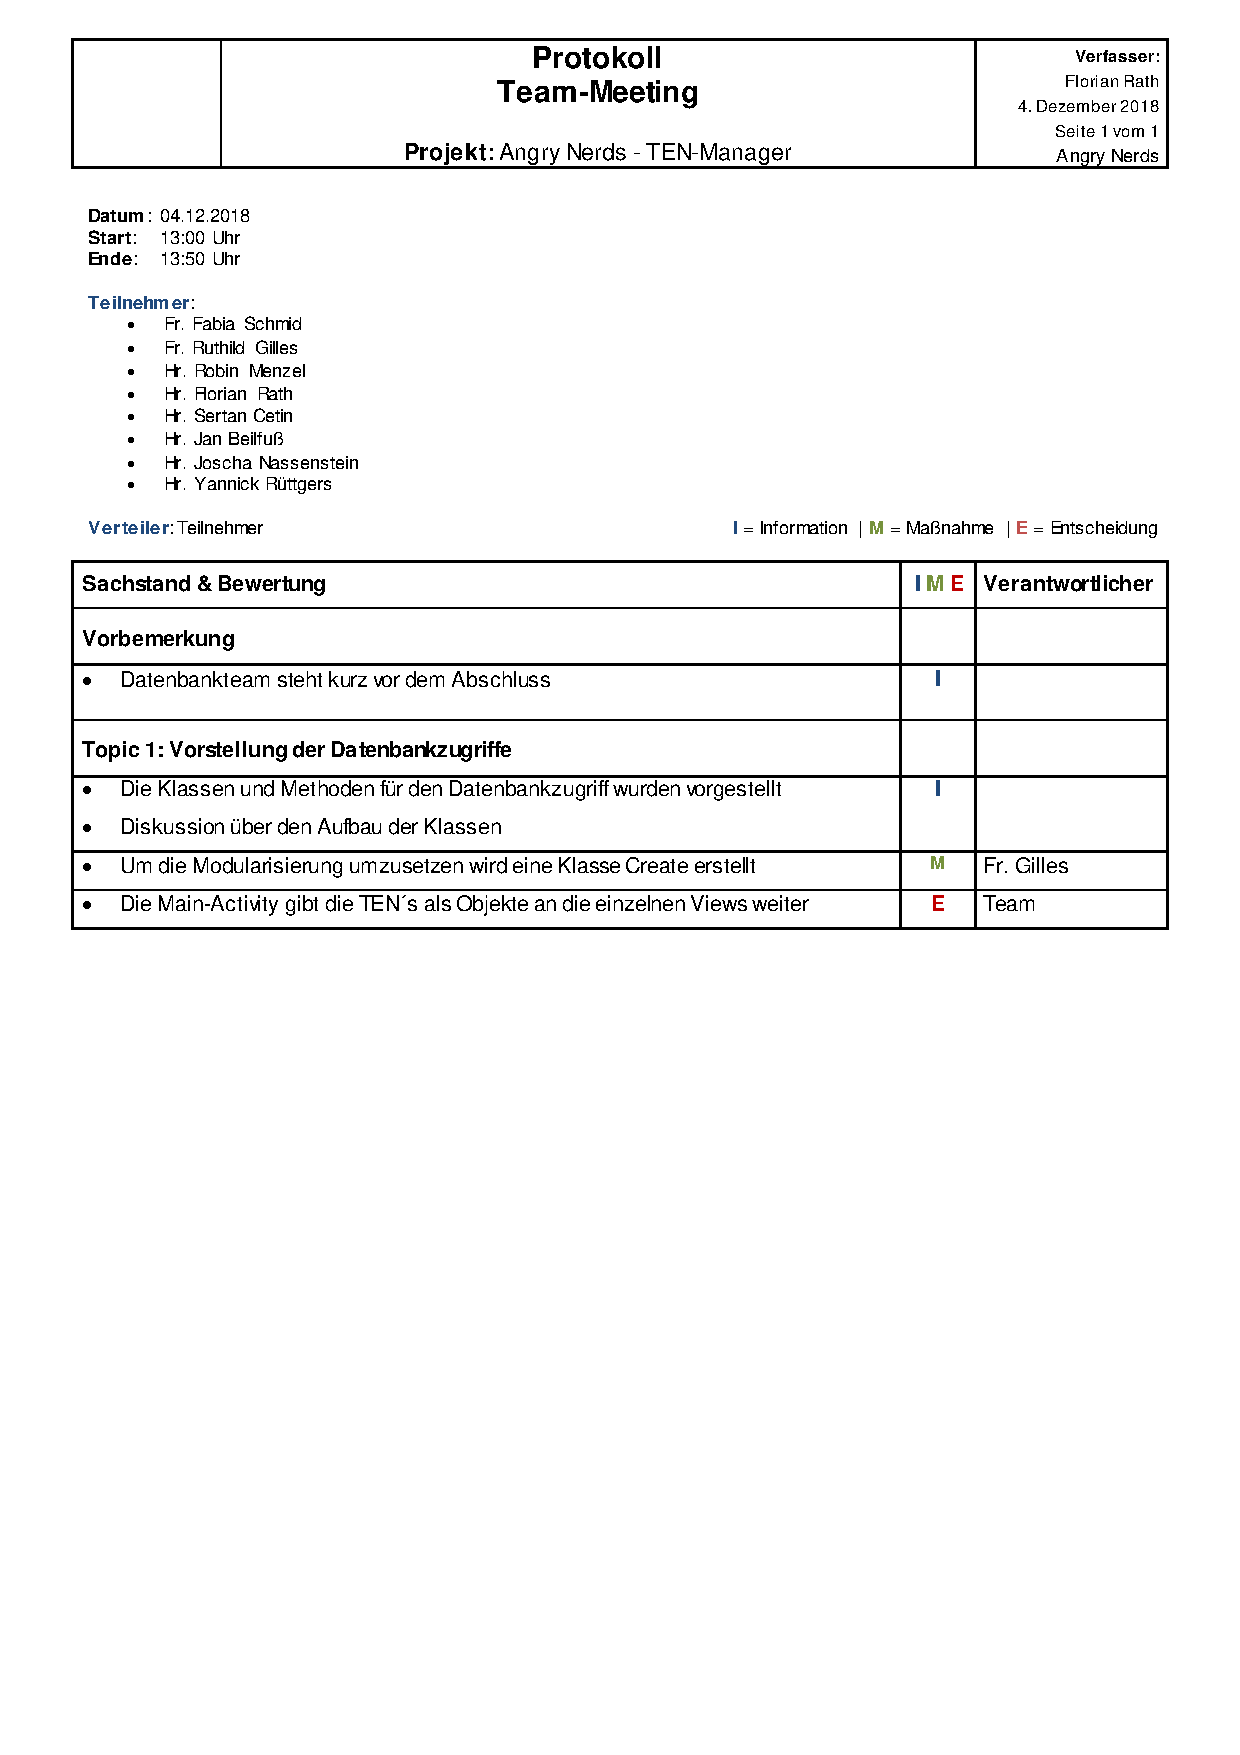
\includegraphics[width=1\textwidth]{img/Protokoll2018-12-04.pdf}\\ % Pfad
\end{minipage}
\end{figure}

\subsection{Projekttagebücher aller Teammitglieder}
%%%%%%%%%%%
%Ruthild
%%%%%%%%%%%
\subsubsection{Projekttagebuch Jan Beilfuß}
\begin{longtable}{|p{10cm}|p{2cm}|p{2cm}|}
\hline
{\textbf{Beschreibung}} & {\textbf{Dauer}} & {\textbf{Datum}} \\ \hline
Aufgabe lesen und verstehen                                                              & 30 min                                & 05.09.2018                            \\ \hline
		Kick-Off-Meeting zur Besprechung der Aufgabe, Verteilung der Rollen                      & 50 min                                & 05.09.2018                            \\ \hline
		Festlegung des Umfangs (Muss/Kann-Kriterien) / Erarbeitung der Eigenschaften von TENs    & 50 min                                & 05.09.2018                            \\ \hline
		Besprechung der in Aufgabenteilung entstandenen Ergebnisse                               & 40 min                                & 05.09.2018                            \\ \hline
		Installation von LateX                                                                   & 60 min                                & 10.09.2018                            \\ \hline
		Erste Überlegungen zum Datenhandling/Datenmodell                                         & 20 min                                & 11.09.2018                            \\ \hline
		Erste Recherche Datenbanken in Android                                                   & 30 min                                & 11.09.2018                            \\ \hline
		Erstellung Datenbankmodell für relationale Datenbank                                     & 50 min                                & 15.09.2018                            \\ \hline
		Team-Meeting Projektteam                                                                 & 40 min                                & 22.09.2018                            \\ \hline
		Weitere Recherche Datenbanken mit Android (Dokumentenbasierte Datenbanken)               & 60 min                                & 22.09.2018                            \\ \hline
		Recherche Couchbase (inkl. Dependency Injection)                                         & 60 min                                & 06.10.2018                            \\ \hline
		Planung Data Layer Architektur                                                           & 20 min                                & 22.10.2018                            \\ \hline
		Anlegen Packagestruktur Struktur (Service/Repository)                                    & 10 min                                & 22.10.2018                            \\ \hline
		Teammeeting Data-Team                                                                    & 60 min                                & 26.10.2018                            \\ \hline
		Git: Anlegen Branches für Joscha und Ruthild                                             & 10 min                                & 26.10.2018                            \\ \hline
		Git Versuch IDEA-Files aus Repository zu entfernen (gescheitert)                         & 60 min                                & 27.10.2018                            \\ \hline
		Telefonat mit Ruthild: Unterstützung bei der IDEA und Git-Einrichtung                    & 120 min                               & 27.10.2018                            \\ \hline
		Erstellung Protokoll Team-Meeting Data-Team vom 26.10.2018                               & 20 min                                & 30.10.2018                            \\ \hline
		Erstellung des Projekttagebuchs                                                          & 20 min                                & 30.10.2018                            \\ \hline
		Teammeeting Data-Team                                                                    & 100 min                               & 20.11.2018                            \\ \hline
		Couchbase - Experimente (Nested Arrays und Objects)                                      & 120 min                               & 23.11.2018                            \\ \hline
		Couchbase - Einarbeitung Object (De)serialization with Jackson                           & 40 min                                & 13.12.2018                            \\ \hline
		Git Repository neu aufsetzen (Merger und neu anlegen)                                    & 180 min                               & 01.12.2018                            \\ \hline
		Erstellung Grafik Softwarearchitektur                                                    & 30 min                                & 06.12.2018                            \\ \hline
		Couchbase Recherche - Views und Queries                                                  & 20 min                                & 17.12.2018                            \\ \hline
		Erstellung des Projekttagebuchs                                                          & 10 min                                & 19.12.2018                            \\ \hline
		Implementierung der ersten schreibenden Zugriffe auf die Datenbank (inklusive Converter) & 160 min                               & 07.01.2019                            \\ \hline
		Implementierung der Deserialisierung/Serialisierung                                      & 150 min                               & 08.01.2019                            \\ \hline
		Optimierung des Jackson-Einsatzes mit @JsonIgnore                                        & 20 min                                & 09.01.2019                            \\ \hline
		Implementierung der Einzelzugriffe auf die Datenbank                                     & 100 min                               & 11.01.2019                            \\ \hline
		Implementierung der Query getAllTENS + Testumgebung                                      & 70 min                                & 12.01.2019                            \\ \hline
		Optimierung Struktur und Bugfixing Repository                                            & 50 min                                & 13.01.2019                            \\ \hline
		Implementierung: Speicherung der Bilder als BLOB in der Datenbank                        & 110 min                               & 15.01.2019                            \\ \hline
		Implementierung asynchrone Ladelogik in Note zum Laden von Bildern                       & 160 min                               & 16.01.2019                            \\ \hline
		Debugging Bilderspeicherung inkl. Evaluation alternativer Speichermöglichkeiten          & 60 min                                & 17.01.2019                            \\ \hline
		Erste Strukturänderungen in Note: Ladeprozess der Note                                   & 120 min                               & 18.01.2019                            \\ \hline
		Unterstützung git bei Todo Leuten                                                        & 60 min                                & 19.01.2019                            \\ \hline
		Implementierung FileRepository                                                           & 180 min                               & 19.01.2019                            \\ \hline
		Debugging FileRepository                                                                 & 60 min                                & 20.01.2019                            \\ \hline
		Erneute Anpassung Repositorystruktur                                                     & 50 min                                & 21.01.2019                            \\ \hline
		Bugfixing und Unterstützung Yannick Rüttgers beim Laden der Bilder                       & 40 min                                & 25.01.2019                            \\ \hline
		Bugfixing getAllTENs Query                                                               & 20 min                                & 25.01.2019                            \\ \hline
		Festlegung von BundleKeys für TEN-Objekte                                                & 10 min                                & 25.01.2019                            \\ \hline
		Unterstützung git bei Todo Leuten                                                        & 80 min                                & 26.01.2019                            \\ \hline
		Reorganisation Note Data                                                                 & 170 min                               & 26.01.2019                            \\ \hline
		Reorganisation Note ApplicationLogic und Data                                            & 210 min                               & 27.01.2019                            \\ \hline
		Umstellung des Bilderhandlings in Note auf den Tablet RAM                                & 110 min                               & 28.01.2019                            \\ \hline
		Weitergehende Speicherplatzoptimierung und damit einhergendes Bugfixing                  & 130 min                               & 29.01.2019                            \\ \hline
		Implementierung der Bildkompression bei großen Gallerieimporten                          & 60 min                                & 30.01.2019                            \\ \hline
		Tabletbeschaffung                                                                        & 10 min                                & 31.01.2019                            \\ \hline
		Implementierung Configuration Change beim ImageOverlay                                   & 80 min                                & 02.02.2019                            \\ \hline
		Testing für Activities auf Tablet                                                        & 100 min                               & 02.02.2019                            \\ \hline
		Dokumentation des Projektes                                                              & 120 min                               & 02.02.2019                            \\ \hline
		Testing der App auf dem Tablet                                                           & 50 min                                & 03.02.2019                            \\ \hline
		Dokumentation des Projektes                                                              & 480 min                               & 03.02.2019                            \\ \hline
\end{longtable}
Summe in Minuten: 4380

\newpage
\subsubsection{Projekttagebuch Joscha Nassenstein}
\begin{longtable}{|p{10cm}|p{2cm}|p{2cm}|}
\hline
{\textbf{Beschreibung}} & {\textbf{Dauer}} & {\textbf{Datum}} \\ \hline
Aufgabe lesen und verstehen & 30 min & 05.09.2018 \\ \hline
Kick-Off Meeting zur Besprechung der Aufgabe, Verteilung der Rollen & 50 min & 05.09.2018 \\ \hline
Festlegung des Umfangs (Muss/Kann-Kriterien) & 50 min & 05.09.2018 \\ \hline
Besprechung der in Aufgabenteilung entstandenen Ergebnisse & 40 min & 05.09.2018 \\ \hline
Übertragung der Ergebnisse in Microsoft Teams & 10 min & 05.09.2018 \\ \hline
Wahl der LaTeX Distribution & 20 min & 12.09.2018 \\ \hline
Download und Installation von LaTeX & 80 min & 12.09.2018 \\ \hline
Erstellung des Datenmodells & 50 min & 15.09.2018 \\ \hline
Digitalisierung des Datenmodells & 20 min & 15.09.2018 \\ \hline
Team-Meeting & 60 min & 22.09.2018 \\ \hline
Erstellung eines GitHub Accounts & 10 min & 13.10.2018 \\ \hline
Installation und Einrichtung von GIT & 30 min & 13.10.2018 \\ \hline
Absprache zur Vererbungsstruktur innerhalb des Data-Layers  & 20 min & 23.10.2018 \\ \hline
Besprechung der Aufgabenverteilung im Data-Team & 60 min & 26.10.2018 \\ \hline
Besprechung der Layouts & 30 min & 27.10.2018 \\ \hline
Pull des aktuellen Stands des Projekts aus dem Repository auf GitHub & 10 min & 28.10.2018 \\ \hline
Implementierung der Klassen TEN sowie der daraus abgeleiteten Klassen ToDo, Event, Note sowie zugehörigen Models & 80 min & 28.10.2018 \\ \hline
Anpassung von colors.xml  & 10 min & 28.10.2018 \\ \hline
Veränderung der Art der Übergabe von Farbwerten aus colors.xml in oben genannte Klassen & 30 min & 28.10.2018 \\ \hline
Erstellung von Beispieldaten (ToDos, Events und Notizen) & 40 min & 30.10.2018 \\ \hline
Erstellung des Projekttagebuchs in Latex & 30 min & 30.10.2018 \\ \hline
Update der TEN-Klassen & 30 min & 17.11.2018 \\ \hline
Merge der GIT-Branches & 10 min & 20.11.2018 \\ \hline
Besprechung Data-Team& 60 min & 20.11.2018 \\ \hline
Erstellung Klassendiagramm& 20 min & 20.11.2018 \\ \hline
Besprechung Team Todo und Note& 80 min & 22.11.2018 \\ \hline
Team-Meeting& 50 min & 04.12.2018 \\ \hline
Besprechung der Anforderungen und der Implementierung von Todo und Note& 150 min & 18.12.2018 \\ \hline
Besprechung der Aufteilung zwischen Todo und Note, Übernahme der Note Activity& 20 min & 21.12.2018 \\ \hline
Design der Layouts für die Note Activity& 200 min & 27.12.2018 \\ \hline
Übernahme der Klassenstruktur aus der Vorlesung und Beginn der Implementation& 400 min & 28.12.2018 \\ \hline
Implementierung der Bildanzeige in der Vorschauansicht& 250 min & 29.12.2018 \\ \hline
Implementierung der Bildanzeige auf Vollbildschirm& 200 min & 29.12.2018 \\ \hline
Implementierung der Datenhaltung bei Konfigurationsänderung & 80 min & 29.12.2018 \\ \hline
Implementierung des Bildimports & 280 min & 30.12.2018 \\ \hline
Erstellung der Layouts für die NoteTagActivity& 120 min & 30.12.2018 \\ \hline
Implementierung der NoteTagActivity & 320 min & 31.12.2018 \\ \hline
Implementierung des Austauschs zwischen den Activities& 80 min & 31.12.2018 \\ \hline
Verbesserung des ImageOverlays& 60 min & 07.01.2019 \\ \hline
Verbesserung des Landscape-Layouts& 140 min & 07.01.2019 \\ \hline
Verbesserung der Fehlertoleranz& 90 min & 08.01.2019 \\ \hline 
Implementierung der Toolbar& 80 min & 11.01.2019 \\ \hline 
Update des Layouts mittels Separatoren& 40 min & 13.01.2019 \\ \hline 
Änderung von Klassenattributen auf zentral angelegte Konstanten& 40 min & 13.01.2019 \\ \hline 
Umbenennung einiger Variablen zur Erhöhung der Lesbarkeit& 60 min & 14.01.2019 \\ \hline 
Implementierung der Bildkorrektur für ein korrekt ausgerichtetes Bild& 120 min & 16.01.2019 \\ \hline 
Implementierung der Teilen-Funktion& 50 min & 17.01.2019 \\ \hline 
Erweiterung der Suchfunktion auf Stichworte& 20 min & 18.01.2019 \\ \hline 
Anpassung des Bildimports an Android API 19& 50 min & 18.01.2019 \\ \hline 
Implementierung der Wischgeste für die Bildvorschau& 240 min & 20.01.2019 \\ \hline 
Erstellung der Dokumentation & 100 min & 02.02.2019 \\ \hline
Erstellung des Projekttagebuchs in Latex & 50 min & 02.02.2019 \\ \hline
Erstellung der Dokumentation & 160 min & 03.02.2019 \\ \hline
\end{longtable}
Summe in Minuten: 4410

\newpage
\subsubsection{Projekttagebuch Fabia Schmid}
\begin{longtable}{|p{10cm}|p{2cm}|p{2cm}|}
\hline
{\textbf{Beschreibung}} & {\textbf{Dauer}} & {\textbf{Datum}} \\ \hline
Aufgabe lesen und verstehen & 30 min & 05.09.2018 \\ \hline
Kick-Off Meeting zur Besprechung der Aufgabe, Verteilung der Rollen & 50 min & 05.09.2018 \\ \hline
Erstellung eines Meilensteinplans & 50 min & 05.09.2018 \\ \hline
Vorstellung des Meilensteinplans und Besprechung der anderen Ergebnisse & 40 min & 05.09.2018 \\ \hline
Aufarbeitung der Abgabetermine und Information der Gruppenteilnehmer  & 20 min & 10.09.2018 \\ \hline
Installation von Latex & 120 min & 10.09.2018 \\ \hline
Festlegung des Vorgehensmodells, durch Abwägung von Vor- und Nachteilen der verschiedenen Modelle (Ergebnis: Erweitertes Wasserfallmodell)
 & 40 min & 11.09.2018 \\ \hline
Teammeeting & 60 min & 22.09.2018 \\ \hline
Github Anmeldung und Einbindung des Projektes & 60 min & 13.10.2018 \\ \hline
Entwicklung des Layouts für das „Event“  & 70 min & 20.10.2018 \\ \hline
Entwicklung des Layouts für das „Note“ & 60 min & 21.10.2018 \\ \hline
Recherche über Listen, Checkboxen und Verwendung von mehreren Layouts & 50 min & 21.10.2018 \\ \hline
Besprechung der Layouts (Aufbau, etc.) & 50 min & 27.10.2018 \\ \hline
Entwicklung des Layouts für das „ToDo“ & 40 min & 27.10.2018 \\ \hline
Erstellung des Projekttagebuch mit Latex & 40 min & 30.10.2018 \\ \hline
Zusammentragung der momentanen Projektstände und Abschätzung, ob die Meilensteine erreicht werden können & 30 min & 17.11.2018 \\ \hline
Neuplanung eines Meilensteins und Abstimmung mit dem Team & 20 min & 26.11.2018 \\ \hline
Teammeeting & 50 min & 04.12.2018 \\ \hline
Koordination der anzufertigen Diagramme und Entwicklungsstand überprüfen & 10 min & 04.12.2018 \\ \hline
Entwicklung des Layouts für das „Image“ & 20 min & 12.12.2018 \\ \hline
Projekttagebuch in Latex führen & 30 min & 19.12.2018 \\ \hline
Entwicklung der Layouts für die Overview & 130 min & 02.01.2019 \\ \hline
Aufteilung der Ausarbeitung & 30 min & 02.01.2019 \\ \hline
Anpassung der OverviewActivity-Layouts & 70 min & 03.01.2019 \\ \hline
Implementierung der Funktion OverviewClickListener & 80 min & 03.01.2019 \\ \hline
Implementierung der Funktion OverviewHeaderClickListener & 60 min & 03.01.2019 \\ \hline
Entwicklung des Layouts für das Bedienleisten-Fragment & 70 min & 04.01.2019 \\ \hline
Implementierung der Funktion OverviewFragmentClickListener & 100 min & 12.01.2019 \\ \hline
Implementierung der Funktion OverviewFragmentLongClickListener & 70 min & 12.01.2019 \\ \hline
Meilenstein Umplanung & 20 min & 15.01.2019 \\ \hline
Layoutanpassung Note Image & 70 min & 18.01.2019 \\ \hline
Erinnerung an die Erstellung der Kapitel der Ausarbeitung & 10 min & 23.01.2019 \\ \hline
Layoutanpassungen OverviewActivity & 120 min & 26.01.2019 \\ \hline
Erstellunng des GANTT-Diagramms & 60 min & 01.02.2019 \\ \hline
Erstellung der Aufgaben-Tabellen in Latex & 110 min & 02.02.2019\\ \hline
Anpassung des Event-Layouts & 60 min & 02.02.2019 \\ \hline
Anpassung des ToDo-Layouts & 80 min & 02.02.2019 \\ \hline
Anpassung der Buttons zum Filtern & 90 min & 03.02.2019 \\ \hline
Dokumentation & 420 min & 03.02.2019 \\ \hline
Projekttagebuch in Latex führen & 30 min & 03.02.2019 \\ \hline
\end{longtable}
Summe in Minuten: 2620

\newpage
\subsubsection{Projekttagebuch Florian Rath}
\begin{longtable}{|p{10cm}|p{2cm}|p{2cm}|}
\hline
{\textbf{Beschreibung}} & {\textbf{Dauer}} & {\textbf{Datum}} \\ \hline
Aufgaben lesen und verstehen & 30 min & 05.09.2018\\ \hline 
Kick-Off Meeting zur Besprechung der Aufgabe, Verteilung der Rollen & 50 min & 05.09.2018\\ \hline 
Erstellung eines Mockups & 50 min & 05.09.2018\\ \hline 
Besprechung der in Aufgabenteilung entstandenen Ergebnisse & 40 min & 05.09.2018\\ \hline 
Installation von LateX & 40 min & 11.09.2018\\ \hline 
Beginn der Planung Navigation zwischen Activities & 50 min & 11.09.2018\\ \hline 
Teammeeting & 60 min & 22.09.2018\\ \hline 
Rollenzuordnung der Activities & 60 min & 01.10.2018\\ \hline 
Bekanntmachung der Zuordnung und Anpassung & 30 min & 02.10.2018\\ \hline 
Installation und Einrichtung von GIT & 30 min & 13.10.2018\\ \hline 
Besprechung der Layouts & 30 min & 27.10.2018\\ \hline 
Beschäftigung mit LateX und Recherche & 100 min & 29.10.2018\\ \hline 
Besprechung Team Todo und Note & 80 min & 22.11.2018\\ \hline 
Team-Meeting & 50 min & 04.12.2018\\ \hline 
Nachbearbeitung Meetingprotokoll und Upload & 30 min & 04.12.2018\\ \hline 
Teilimplementation Todo und Note & 150 min & 18.12.2018\\ \hline 
Beschäftigung mit Datepicker für Todo & 240 min & 04.01.2019\\ \hline 
Implementierung der Colors und Start-/Enddatum & 280 min & 21.01.2019\\ \hline 
Layoutanpassungen & 250 min & 22.01.2019\\ \hline 
Layoutanpassungen und Funktionalitäten für Todo & 290 min & 26.01.2019\\ \hline 
Bug fixes und weitere Funktionalitäten für Todo & 310 min & 30.01.2019\\ \hline 
Dokumentation & 280 min & 03.02.2019\\ \hline 
\end{longtable}
Summe in Minuten: 2530

\newpage
\subsubsection{Projekttagebuch Robin Menzel}
\begin{longtable}{|p{10cm}|p{2cm}|p{2cm}|}
\hline
{\textbf{Beschreibung}} & {\textbf{Dauer}} & {\textbf{Datum}} \\ \hline
Aufgabe lesen und verstehen & 30 min & 05.09.2018 \\ \hline
Kick-Off Meeting zur Besprechung der Aufgabe, Verteilung der Rollen & 50 min & 05.09.2018 \\ \hline
Konzeption eines Mockups und den Activities & 50 min & 05.09.2018 \\ \hline
Besprechung der in Aufgabenteilung entstandenen Ergebnisse & 40 min & 05.09.2018 \\ \hline
Installation von Adobe XD für MockUps & 20 min & 05.09.2018 \\ \hline
Installation und Einrichtung von Git & 20 min & 05.09.2018 \\ \hline
Erstellung und Einrichtung eines GitHub Repositorys & 40 min & 05.09.2018 \\ \hline
Erstellung von MockUps in der ersten Version & 180 min & 06.09.2018 \\ \hline
Wahl der LateX Distribution & 20 min & 10.09.2018 \\ \hline
Installation von LateX & 120 min & 10.09.2018 \\ \hline
Projekttagebuch pflegen & 10 min & 11.09.2018\\ \hline
Weiterentwicklung des MockUps & 30 min & 15.09.2018\\ \hline
Meeting zur Besprechung der Ergebnisse aus dem Design- und Daten-Team & 60 min & 22.09.2018\\ \hline
Korrekturen am MockUp und Teilen der Ergebnisse im Microsoft Teams & 30 min & 23.09.2018\\ \hline
Kommunikation mit Data Team im Bezug auf Objekte und Übergabe an Activities & 30 min & 23.10.2018 \\ \hline
Erstellung des XML-Layouts der Event-Activity & 180 min & 27.10.2018\\ \hline
Recherche und Design von Farben für die Hintergründe von Activities und Erstellung von res-Files & 60 min & 28.10.2018\\ \hline
Probleme im Git Repository beheben und einrichten von Branches & 30 min & 28.10.2018\\ \hline
Erstellung des Projekttagebuchs in Latex & 40 min & 30.10.2018 \\ \hline
Weiterentwicklung des XML-Layouts der Event-Activity & 120 min & 15.10.2018\\ \hline
Recherche Umsetzung der Datumsauswahl (DatePicker) & 60 min & 15.10.2018\\ \hline
Git Repository neu aufsetzen (Merger und neu anlegen) & 180 min & 01.12.2018\\ \hline
Teammeeting & 50 min & 04.12.2018\\ \hline
Erstellung Notwendiger Klassen für die Event Activity & 600 min & 10.12.2018 \\ \hline
Recherche nach App oder Toolbar für API 19 & 120 min & 12.12.2018 \\ \hline
Implementation einer Toolbar für alle TENs & 260 min & 13.12.2018 \\ \hline
Implementation des 3-Punkt-Menüs in der Toolbar & 30 min & 13.12.2018 \\ \hline
Implementation des Öffnens der Activity (Öffnen mit ID, ohne, Übergänge) & 90 min &  17.12.2018\\ \hline
Erstellung des Projekttagebuchs in Latex & 15 min & 19.12.2018 \\ \hline
Recherche DialogPicker um Zeit und Datum für Events auszuwählen & 120 min & 23.12.2018 \\ \hline
Implementation von Date- und Time-Picker & 300 min & 27.12.2018 \\ \hline
Implementation der dynamischen Reminder in der GUI und dem Auswahldialog & 390 min & 29.12.2018 \\ \hline
Recherche Notification Service und Alarm Manager & 90 min & 30.12.2019 \\ \hline
Implementation von Remindern inkl. Notification Service und Alarm Manager & 120 min & 31.01.2019 \\ \hline
Ausführliches Testen 05.01.2019 & 120 min & 04.01.2019\\ \hline
Anpassungen auf API 19 & 120 min & 05.01.2019 \\ \hline
Ausführliches Testen 09.01.2019 & 90 min & 10.01.2019\\ \hline
Anpassungen an dem Alarm Manager um Reminder vor aktueller Zeit zu ignorieren & 30 min & 10.01.2019 \\ \hline
Recherche nach Schnittstellen zu Google Maps & 15 min & 10.01.2019 \\ \hline
Implementation eines Buttons um die Adresse eines Events in Google Maps zu öffnen & 30 min 6 & 10.01.2019 \\ \hline
GUI Anpassungen für den Navigations-Button & 30 min & 11.01.2019 \\ \hline
Implementation einer Teilen-Funktionalität für Text-basiertes Event & 45 min & 13.01.2019 \\ \hline
Implementation einer Export-Funktion in andere Kalender Applikationen & 30 min & 13.01.2019 \\ \hline
Implementation der Wiederholungsfunktion (Einmalig, Täglich, ...) & 180 min & 17.01.2019 \\ \hline
Erstellung der Dokumentation 1 & 120 min & 28.01.2019 \\ \hline
Erstellung des Projekttagebuchs in Latex & 60 min & 29.12.2018 \\ \hline
Erstellung der Dokumentation 2 & 140 min & 30.01.2019 \\ \hline
\end{longtable}
Summe in Minuten: 4595

\newpage
\subsubsection{Projekttagebuch Ruthild Gilles}
\begin{longtable}{|p{10cm}|p{2cm}|p{2cm}|}
\hline
{\textbf{Beschreibung}} & {\textbf{Dauer}} & {\textbf{Datum}} \\ \hline
Aufgabe lesen und verstehen & 30 min & 05.09.2018 \\ \hline
Kick-Off Meeting zur Besprechung der Aufgabe, Verteilung der Rollen & 50 min & 05.09.2018 \\ \hline
Festlegung des Umfangs (Muss/Kann Kriterien) & 50 min & 05.09.2018 \\ \hline
Besprechung der in Aufgabenteilung entstandenen Ergebnisse & 40 min & 05.09.2018 \\ \hline
Installation von LateX & 120 min & 10.09.2018 \\ \hline
Projekttagebuch ausfüllen & 10 min & 11.09.2018 \\ \hline
Erstellung des Datenmodells & 50 min & 15.09.2018 \\ \hline
Teammeeting & 60 min & 22.09.2018 \\ \hline
Überlegung Aufgabenteilung, Aufgabenvergabe und Erklärung dieser bezogen auf die MainActivity & 40 min & 09.10.2018 \\ \hline
Installation und Einrichtung von GIT & 30 min & 13.10.2018 \\ \hline
Teammeeting Data-Team &  60 min & 26.10.2018 \\ \hline
Klonen des Data-Branches von GIT & 120 min & 27.10.2018 \\ \hline
Deklaration von gettern und settern für Datenobjekte & 120 min & 28.10.2018 \\ \hline
Projekttagebuch ausfüllen & 20 min & 31.10.2018 \\ \hline
Entwicklung von SetterService Klasse & 180 min & 16.11.2018 \\ \hline
Teammeeting Data-Team & 100 min & 20.11.2018 \\ \hline
Entwicklung von Service Klassen & 120 min & 21.11.2018 \\ \hline
Überlegung neuer Struktur für Services & 90 min & 22.11.2018 \\ \hline
Implementierung neuer Service-Struktur & 120 min & 30.11.2018 \\ \hline
Einbindung der Mockdaten & 80 min & 01.12.2018 \\ \hline
Implementierung weiterer Teile neuer Struktur & 90 min & 02.12.2018 \\ \hline
Änderungen an neuer Service-Struktur & 40 min & 03.12.2018 \\ \hline
Teammeeting & 50 min & 04.12.2018 \\ \hline
Entwicklung von Create-Klasse & 60 min & 04.12.2018 \\ \hline
Änderungen an Update-Klasse & 40 min & 17.12.2018 \\ \hline
Projekttagebuch ausfüllen & 20 min & 18.12.2018 \\ \hline
Bugfixing in Update- und Read-Klasse & 90 min & 02.01.2019 \\ \hline
Mockdaten durch Zugriff auf Datenbank ersetzt & 60 min & 02.01.2019 \\ \hline
Ergänzung einer Methode in Delete-Klasse & 30 min & 04.01.2019 \\ \hline
Neue Farben für GUI festlegen & 30 min & 07.01.2019 \\ \hline
Latex - Vorlage anpassen & 120 min & 14.01.2019 \\ \hline
Latex - Struktur für Ausarbeitung erstellen & 120 min & 18.01.2019 \\ \hline
Meinen Teil der Ausarbeitung schreiben & 180 min & 28.01.2019 \\ \hline
Latex - Meetingprotokolle einfügen & 180 min & 01.02.2019 \\ \hline
Latex - Quellcode einfügen & 240 min & 02.02.2019 \\ \hline
Latex - Ausarbeitungen der anderen einfügen & 240 min & 03.02.2019 \\ \hline
Projekttagebuch ausfüllen & 20 min & 03.02.2019 \\ \hline
Latex - Projekttagebücher einfügen & 120 min & 03.02.2019 \\ \hline
\end{longtable}
Summe in Minuten: 3370

\newpage
\subsubsection{Projekttagebuch Sertan Cetin}
\begin{longtable}{|p{10cm}|p{2cm}|p{2cm}|}
\hline
{\textbf{Beschreibung}} & {\textbf{Dauer}} & {\textbf{Datum}} \\ \hline
Aufgaben lesen und verstehen & 30 min & 05.09.2018\\ \hline 
Kick-Off Meeting zur Besprechung der Aufgabe, Verteilung der Rollen & 50 min & 05.09.2018\\ \hline 
Erstellung eines Mockups & 50 min & 05.09.2018\\ \hline 
Besprechung der in Aufgabenteilung entstandenen Ergebnisse & 40 min & 05.09.2018\\ \hline 
Installation von LateX & 40 min & 11.09.2018\\ \hline 
Beginn der Planung Navigation zwischen Activities & 50 min & 11.09.2018\\ \hline 
Teammeeting & 60 min & 22.09.2018\\ \hline 
Rollenzuordnung der Activities & 60 min & 01.10.2018\\ \hline 
Bekanntmachung der Zuordnung und Anpassung & 30 min & 02.10.2018\\ \hline 
Installation und Einrichtung von GIT & 20 min & 13.10.2018\\ \hline 
Besprechung der Layouts & 30 min & 27.10.2018\\ \hline 
Beschäftigung mit LateX und Recherche & 90 min & 29.10.2018\\ \hline 
Erstellung des Projekttagebuchs in LateX & 20 min & 30.10.2018\\ \hline 
Besprechung Team Todo und Note & 80 min & 22.11.2018\\ \hline 
Team-Meeting & 50 min & 04.12.2018\\ \hline 
Teilimplementation Todo und Note & 150 min & 18.12.2018\\ \hline 
Vertiefung von androidspezifischen Controls & 60 min & 19.12.2018\\ \hline 
Erstellung des Projekttagebuchs in LateX & 20 min & 19.12.2018\\ \hline 
Layout für Task Todos & 180 min & 03.01.2019\\ \hline 
Implementierung Taskadapter (Schnittstelle zwischen Gui und Data) & 300 min & 04.01.2019\\ \hline
Bugfixes für Todo Tasks Listview & 120 min & 05.01.2019\\ \hline
Emulator Problembehebung (gescheitert) & 120 min & 21.01.2019\\ \hline 
Implementierung Todo Data und Progresstext & 200 min & 28.01.2019\\ \hline
Implementierung ShareFunktion Todo & 180 min & 02.02.2019\\ \hline
Diverse Bugfixes in Todo Funktionen & 210 min & 03.02.2019\\ \hline
Dokumentation & 180 min & 03.02.2019\\ \hline
\end{longtable}
Summe in Minuten: 2720

\newpage
\subsubsection{Projekttagebuch Yannick Rüttgers}
\begin{longtable}{|p{10cm}|p{2cm}|p{2cm}|}
\hline
{\textbf{Beschreibung}} & {\textbf{Dauer}} & {\textbf{Datum}} \\ \hline
Aufgabe lesen und verstehen & 30 min & 05.09.2018\\ \hline 
Kick-Off Meeting zur Besprechung der Aufgabe, Verteilung der Rollen & 50 min & 05.09.2018\\ \hline 
Erstellung eines Meilensteinplans & 50 min & 05.09.2018\\ \hline 
Besprechung der in Aufgabenteilung entstandenen Ergebnisse & 40 min & 05.09.2018\\ \hline 
Wahl der Latex Distribution & 20 min & 10.09.2018\\ \hline 
Installation von Latex & 120 min & 10.09.2018\\ \hline 
Festlegung des Vorgehensmodells & 20 min & 11.09.2018\\ \hline 
Meeting zur Besprechung der Ergebnisse aus dem Design- und Daten-Team & 60 min & 22.09.2018\\ \hline 
Recherche Technologie "Fragments & 90 min & 07.10.2018\\ \hline 
Entwicklung einer Testapplikation mit Fragments, Beschäftigung mit dem Lifecycle derer & 120 min & 08.10.2018\\ \hline 
Überlegung Aufgabenteilung, Aufgabenvergabe und Erklarung dieser bezogen auf die MainActivity & 40 min & 09.10.2018\\ \hline 
Installation und Einrichtung von GIT & 30 min & 13.10.2018\\ \hline 
Provisorische Startseite fürs Development & 60 min & 20.10.2018\\ \hline 
Kommunikation mit Data Team im Bezug auf Objekte und Übergabe an Activities & 30 min & 23.10.2018\\ \hline 
Besprechung der Layouts & 30 min & 27.10.2018\\ \hline 
Erstellung des Projekttagebuchs in Latex & 40 min & 29.10.2018\\ \hline 
Weitere Beschaftigung mit Latex & 90 min & 29.10.2018\\ \hline 
Teammeeting & 50 min & 04.12.2018\\ \hline 
Beratung bei der Erstellung weiterer Layouts & 30 min & 12.12.2018\\ \hline 
Erstellung von Coding Conventions & 50 min & 14.12.2018\\ \hline 
Hinzufügen der Layouts in das Projekt, Anpassen der Layouts an Coding Conventions & 140 min & 18.12.2018\\ \hline 
Klassenstruktur der Activity Overview planen & 200 min & 28.12.2018\\ \hline 
Erschaffen der Grundstruktur für die Hauptactivity & 180 min & 28.12.2018\\ \hline 
Implementierung des Datenmodells der Activity & 50 min & 30.12.2018\\ \hline 
Implementierung der GUI und des Controllers der Activity & 70 min & 30.12.2018\\ \hline 
Schaffung einer Verbindung zwischen den Schichten & 60 min & 30.12.2018\\ \hline 
Korrektur der Mockdaten & 20 min & 30.12.2018\\ \hline 
Vorbereitung eines Beispielfragments & 30 min & 31.12.2018\\ \hline 
Hinzufügen eines Fragments in die Container der Übersicht & 120 min & 31.12.2018\\ \hline 
Planung der Datenübertragung zwischen Fragment und Activity & 110 min & 01.01.2019\\ \hline 
Implementierung von Bundles in den Datenklassen & 60 min & 01.01.2019\\ \hline 
Implementierung des Notefragments & 120 min & 02.01.2019\\ \hline 
Planung und Entwicklung von Superklassen für die Fragments  & 160 min & 02.01.2019\\ \hline 
Bugfixing bezogen auf das Neuerstellen von Fragments bei Verändern der Konfiguration & 120 min & 03.01.2019\\ \hline 
Implementierung von Fragmenthelferklassen & 120 min & 03.01.2019\\ \hline 
Update des OverviewLayouts & 60 min & 03.01.2019\\ \hline 
Planung der Löschfunktionalität & 70 min & 03.01.2019\\ \hline 
Implementation der Löschfunktionalität & 120 min & 03.01.2019\\ \hline 
Implementierung des Markierungsprozesses & 40 min & 04.01.2019\\ \hline 
Implementierung von Helferklassen für den Löschprozess & 60 min & 04.01.2019\\ \hline 
Planung und Implementierung des Layoutwechsels bei Veränderung der Orientierung & 80 min & 04.01.2019\\ \hline 
Implementation Event Fragment & 60 min & 04.01.2019\\ \hline 
Implementierung Todofragment ohne Tasks & 60 min & 04.01.2019\\ \hline 
Implementierung der Tasks & 80 min & 05.01.2019\\ \hline 
Testing der Fragments & 60 min & 05.01.2019\\ \hline 
Bugfixing Löschprozess & 80 min & 25.01.2019\\ \hline 
Planung und Implementierung der Öffnung von TENs & 60 min & 25.01.2019\\ \hline 
Bugfixing Adresse in Event & 20 min & 25.01.2019\\ \hline 
Implementierung des ImageFragments & 210 min & 25.01.2019\\ \hline 
Implementierung einer Highlightfunktionalität für Leiste am unteren Bildschirmrand & 20 min & 26.01.2019\\ \hline 
Anpassen von Bundleids an Konstanten & 20 min & 26.01.2019\\ \hline 
Bugfixing Scrollview & 60 min & 26.01.2019\\ \hline 
Bugfixing Jahr im Eventfragment & 20 min & 26.01.2019\\ \hline 
Anpassung der Sprache & 20 min & 26.01.2019\\ \hline 
Hinzufügen eines adaptiven Layouts je nach Bildschirmgröße & 90 min & 27.01.2019\\ \hline 
Planung und Implementierung einer Suchfunktion & 220 min & 03.02.2019\\ \hline 
Hinzufügen weiterer Kommentare & 50 min & 03.02.2019\\ \hline 
Bugfixing Todoicon & 10 min & 03.02.2019\\ \hline 
Dokumentation des Projekts & 360 min & 03.02.2019\\ \hline 
\end{longtable}
Summe in Minuten: 4540


\newpage
\subsection{Beschreibung von Problemen}

\subsubsection{Probleme von Fabia Schmid}
Im Lauf des Projektes konnten zwei Meilensteine nicht fristgerecht erfüllt werden. Einmal die Fertigstellung der Activities und die Fertigstellung der Dokumentation.
 
Die Fertigstellung der Activities und der Layouts war für den 01.12.2018 geplant, konnte jedoch nicht fristgerecht fertiggestellt werden, da projektfremde Tätigkeiten die Umsetzung verzögerten. Beispielsweise schrieben wir eine Klausur, die bei der Projektplanung noch nicht bekannt war. Als Ergebnis wurde der Meilenstein auf ein späteres Datum geplant und konnte danach fristgerecht erfüllt werden. Diese Verschiebung hatte jedoch keinen negativen Einfluss auf die Fertigstellung des Projektes.

Auch der Meilenstein „Dokumentation fertig“ konnte nicht fristgerecht zum 01.02.2019 erreicht werden. Auch in diesem Fall waren projektfremde Tätigkeiten die Ursache für den Verzug. Jedoch musste der Meilenstein nur um 3 Tage verschoben werden, wodurch das Projektergebnis nicht gefährdet wurde.

Weitere Probleme oder Verzögerungen traten nicht auf und das Projekt konnte erfolgreich am 09.02.2019 vorgestellt werden.

\subsubsection{Probleme von Florian Rath}
Im Zuge der Entwicklung tauchten einige Probleme auf, die unterschiedlichen Ursprüngen entstammten. Zum einen fiel auf, dass die Aufteilung der Entwicklung nach den Activities viel Kommunikation benötigte und einige Klassen redundant erstellt wurden. Die Aufteilung nach Elementen hätte hier sicherlich mehr Sinn gemacht. Dann wären zum Beispiel alle GUI-Klassen von einer Person entwickelt worden. Ein zusätzlicher Faktor für Probleme war die Zeit, da die Entwicklung immer mal wieder unterbrochen wurde, kam man als Entwickler öfter aus dem Tritt.

Die Entwicklung mit Android Studio war in manchen Phasen ebenfalls problembehaftet. Der Emulator ließ sich aus unergründlichen Ursachen nicht starten und musste neuinstalliert werden. Nach manchen Abgleichen mit GitHub wies der Code Fehler auf und konnte nicht mehr kompiliert werden, das Problem ließ sich nur mit einem kompletten Download des Projektes bewerkstelligen.

\subsubsection{Probleme von Jan Beilfuß}
Im Projektverlauf traten einige Probleme auf. Während der Arbeit im Datateam waren die Zwischenergebnisse zu Implementierungsbeginn schwierig zu testen, da diese zum Großteil implementiert wurden, bevor man eine Anbindung an die Activities hatte. Die Suche nach möglichen Fehlern wurde hier hauptsächlich über den Logcat durchgeführt. Dennoch wurden noch Fehler bei der Anbindung der Activities entdeckt und konnten demzufolge erst zu dem Zeitpunkt behoben werden.

Weiterhin hat der Wechsel vom privaten Android-Smarthpone auf das FHDW-eigene Tablet Probleme bereitet. Insbesondere die Kombination aus dem geringen Arbeitsspeicher auf dem Tablet und einem nicht funktionierenden Profiler (dieser soll den Arbeitsspeicherverbrauch loggen) in Android Studio hat das Optimieren des Speicherbedarfs in der Note-Activity erschwert.

\subsubsection{Probleme von Joscha Nassenstein}
Zu Beginn der Entwicklung benötigte es sehr viel Zeit, durch das Implementieren verschiedener Möglichkeiten, beispielsweise für die Stichwortliste, die beste Lösung zu finden. Da ich stets mein eigenes Android-Smartphone, welches zurzeit auf API 29 läuft, für das Testen verwendete, implementierte ich teilweise Lösungen, welche so auf dem Tablet der Hochschule (API 19) nicht in dem Maße funktionierten, wie es auf meinem Gerät der Fall war.

Vor allem im Umgang mit Textfeldern und beim Überschreiben einiger onTouch-Funktionen kam es dabei zu anderen Ergebnissen, als dies vorher der Fall war. Da in dem AndroidStudio-Projekt API-Level 19 bereits voreingestellt war, wurde direkt ein Hinweis angezeigt, falls man eine Funktion nutzen wollte, welche auf dem Level nicht unterstützt wird. Ein weiteres Beispiel ist die Android-eigene Kamerafunktion, welche vor der Android Version Marshmallow (API 23), in welcher spezielle Laufzeit-Berechtigungen eingeführt wurden, eine Berechtigung zum Schreiben und Lesen der Datei mitgegeben werden muss. Auch dies fiel erst auf, als die App auf dem Tablet getestet wurde. Insgesamt mussten nach den Tests einige kleinere Anpassungen vorgenommen werden.

Eine weitere Herausforderung war die Abstimmung der Programmierungsaufgaben, da diese Activity unter zwei Programmierern aufgeteilt wurde. Dies erforderte, falls in der Zwischenzeit Änderungen dazugekommen waren, ein bisschen Einarbeitungszeit, bevor man weiterprogrammieren konnte. Insgesamt ist das Ergebnis und die Performance jedoch sehr zufriedenstellend und durch die Aufteilung konnten sehr viele Aspekte der Activity optimiert werden. Durch Benennungskonventionen und eine neue Paketstruktur sowie die intensive Abstimmung konnte hier ein gutes Ergebnis entstehen.

\subsubsection{Probleme von Ruthild Gilles}
Während des Projektes kam es zu einigen Komplikationen. Dies lag zum einen an fehlender Erfahrung beim Projektmanagement und der Entwicklung, aber auch an fehlenden Kenntnissen von Versionierung über Git und Dokumentation in Latex.

Für mich persönlich war es eine Herausforderung zwischen den anderen Teammitgliedern, die deutlich besser bzw. schneller entwickeln können als ich, nicht unterzugehen. Mir wurden aufgrund meiner wenigen Erfahrung in der Programmierung von Java zu Beginn nur wenige Aufgaben bezüglich Entwicklung zugeteilt. Da andere Projektmitglieder weniger implementieren wollten, wurden ihnen Aufgaben im Projektmanagement übertragen, allerdings blieben nicht viele Aufgaben offen, an denen ich mich beteiligen könnte.

Da die Planungsphase zugegebenermaßen doch recht kurz ausfiel, musste ich während der Implementierung meiner Klassen ausprobieren und öfters Änderungen durchführen. Besonders herausfordernd war hierbei auf die möglichen Anforderungen einzugehen, die während der Entwicklung der Activities auftreten würden. Besonders die Verantwortlichen der Activities erwarteten von mir, dass ich Methoden zum getten und setten von TEN-Objekten implementierte. Allerdings fehlten mir während der ersten Implementation die genauen Anforderungen der Activities, da die jeweiligen Gruppen selbst noch nicht ins Detail geplant hatten, welche Methoden sie benötigen würden. So kam es dazu, dass ich meine wenigen Methoden erneut und erneut implementierte oder Änderungen durchführte.

Ähnlich verlief es auf der Seite der Datenbank. Die Auswahl der Datenbank wurde zwar bereits sehr früh getroffen, jedoch fehlte der verantwortlichen Person zu Beginn das Wissen und auch von dieser Seite hatte ich keine klaren Anforderungen. Deswegen musste ich auch hier häufige Anpassungen vornehmen und es wurde mit der Zeit auch immer mehr Logik meiner Klassen in die Klassen des Repositories ausgelagert, sodass mein Programmierteil im Endeffekt deutlich kleiner aussieht, als er eigentlich war.

Nachdem ich angemerkt hatte, dass ich Zeit übrig hatte und noch in den Activities helfen könnte, wurde mir jedoch mitgeteilt, dass das Erklären der bisherigen Logik und das Beschreiben der benötigten Funktionalitäten länger dauern würde, als die Implementierung durch bereits eingearbeitete Teammitglieder.

Letztendlich wurde mir die Aufgabe des Latex-Verantwortlichen übertragen und so saß ich die letzte Woche vor Abgabe der Dokumentation an der Einarbeitung, Erstellung und Zusammenstellung der schriftlichen Ausarbeitung in Latex.

\subsubsection{Probleme von Sertan Cetin}
Während der Entwicklung sind bei mir diverse Probleme aufgetreten. Ich habe in meinem privaten Rechner einen AMD Ryzen Prozessor, genauso wie in meinem Laptop. Leider war die Konfiguration mit dem Android-Emulator etwas komplizierter, da Ryzen die Hardwarebeschleunigung von Intel nicht unterstützt. Ich musste lange Recherchearbeit durchführen, bis ich einen Emulator zum laufen bekam. Allerdings stürzte dieser während der Entwicklung aus dem Nichts ab, sodass er bis heute immer noch nicht funktioniert. Ich hatte das Projekt von meinem lokalen Rechner komplett gelöscht und neu heruntergeladen. Nichts brachte die Lösung.

Damit ich trotzdem entwickeln konnte, benutzte ich mein eigenes Android-Handy. Jedoch wäre die Entwicklung mit einem Emulator deutlich entspannter gewesen.

In diesem Punkt betrachte ich Android Studio ein wenig als rückschrittig, wenn man fehlerfreie Tools von Visual Studio gewohnt ist. Bei Visual Studio Fehlern konnte ich im Internet viel schneller eine Lösung finden als bei Android Studio.

\subsubsection{Probleme von Yannick Rüttgers}

Die Probleme, denen während des Projektes auftraten, lagen hauptsächlich an der genutzten Entwicklungsumgebung, bzw. der genutzten Software.

Bereits zu Beginn des Moduls funktionierte weder Androidstudio, noch Latex korrekt. Nach dem Kauf eines neuen Laptops funktionierten die Programme zwar soweit, allerdings konnte aufgrund des AMD-Prozessors die Virtualisierung nicht optimal genutzt werden. Dies führte zu langen Wartezeiten und Fehlern beim Starten des Emulators. Durch Nutzung eines externen Smartphones konnte dies schließlich umgangen werden.



